\documentclass[handout]{beamer}
%==============================================================
% Common Beamer Preamble for Course Lectures: Training and Scaling Language Models
%==============================================================

\usepackage[utf8]{inputenc}
\usepackage[T1]{fontenc}
\usepackage{hyperref}
\usepackage{amsmath,amssymb,xcolor,multicol,booktabs,colortbl}
\usepackage{graphicx,listings}
\renewcommand{\figurename}{Figure.}
\renewcommand{\tablename}{Table.}

% ---- TikZ Libraries ----
\usepackage{tikz}
\usetikzlibrary{positioning,arrows.meta,shapes.geometric,calc,fit,backgrounds,decorations.pathreplacing}

% ---- Presentation defaults ----
\setbeamertemplate{navigation symbols}{}
\setbeamersize{text margin left=0.55cm,text margin right=0.55cm}
\setbeamerfont{title}{size=\LARGE,series=\bfseries}
\setbeamerfont{subtitle}{size=\large}

% ---- FontAwesome fallback ----
\IfFileExists{fontawesome5.sty}{%
  \usepackage{fontawesome5}%
}{%
  \providecommand{\faMicrochip}{}%
  \providecommand{\faComments}{}%
  \providecommand{\faTools}{}%
  \providecommand{\faCheckCircle}{}%
  \providecommand{\faExclamationTriangle}{}%
  \providecommand{\faImage}{}%
  \providecommand{\faRobot}{}%
  \providecommand{\faTerminal}{}%
  \providecommand{\faBook}{}%
  \providecommand{\faRedo}{}%
  \providecommand{\faLayerGroup}{}%
  \providecommand{\faCogs}{}%
  \providecommand{\faDatabase}{}%
  \providecommand{\faHdd}{}%
  \providecommand{\faNetworkWired}{}%
}

% ---- Theme Style and Semantic Colors ----
%==============================================================
% Centralized Semantic Color Definitions for LLMs Presentation
%==============================================================

% ---- Base Template / Theme Colors (Aligned with Palette B) ----
\definecolor{themenavy}{RGB}{22,70,102}       % Palette B primary cerulean: #164666
\definecolor{themeblue}{RGB}{22,70,102}       % Primary alias
\definecolor{primarylight}{RGB}{34,92,132}    % Primary light: #225c84
\definecolor{themeteal}{RGB}{0,159,176}       % Accent cyan-teal: #009fb0
\colorlet{main_color}{themenavy}
\colorlet{accent}{themeteal}

\definecolor{accentdark}{RGB}{0,108,120}      % Deep cyan-teal for contrast text
\definecolor{accentlight}{RGB}{56,178,214}    % Slate accent cyan: #38b2d6
\definecolor{leafred}{RGB}{197,93,61}         % Terracotta red for branches/leaves

% ---- Website Panel & Border Neutrals ----
\definecolor{panelbg}{RGB}{237,245,249}       % Course-panel: #edf5f9
\definecolor{panelborder}{RGB}{204,226,238}   % Course-border: #cce2ee

% ---- Code listing style (syntax highlights) ----
\definecolor{deepblue}{RGB}{22,70,102}
\definecolor{deepred}{rgb}{0.6,0,0}
\definecolor{deepgreen}{RGB}{0,135,150}
\definecolor{halfgray}{gray}{0.55}

% ---- Semantic Theme Navy / Cerulean Shades ----
\colorlet{themebluebg}{panelbg}               % Panel #edf5f9
\colorlet{themebluecard}{main_color!8}        % Mild card background fills
\colorlet{themeblueborder}{panelborder}       % Border #cce2ee
\colorlet{themebluemid}{themeteal!60}         % Accent mid-contrast
\colorlet{themebluedraw}{main_color!80}       % Strong outline draws/strokes

% ---- Semantic Secondary Accent Teal Shades ----
\colorlet{accentdarkbg}{themeteal!10}        % Light secondary background fills
\colorlet{accentdarkdraw}{themeteal}         % Secondary outlines/strokes/text/axes

% ---- Functional Colors: Success Green ----
\definecolor{successgreen}{RGB}{55,145,55}
\colorlet{successbg}{successgreen!8}
\colorlet{successdraw}{successgreen!75}

% ---- Functional Colors: Alert Red ----
\definecolor{alertred}{RGB}{197,55,55}
\colorlet{alertbg}{alertred!8}
\colorlet{alertdraw}{alertred!75}

% ---- Functional Colors: Warning Orange ----
\definecolor{warningorange}{RGB}{220,110,30}
\colorlet{warningbg}{warningorange!10}
\colorlet{warningdraw}{warningorange!80}

% ---- Terracotta Red Shades ----
\colorlet{leafredbg}{leafred!12}
\colorlet{leafreddraw}{leafred!80}

% ---- Accent Violet (SWE-bench / observe phases) ----
\definecolor{accentviolet}{RGB}{120,70,180}
\colorlet{accentvioletbg}{accentviolet!10}
\colorlet{accentvioletdraw}{accentviolet!80}

% ---- Post-Training Axis Blue ----
\definecolor{posttrainingblue}{RGB}{40,90,165}
\colorlet{posttrainingbg}{posttrainingblue!8}
\colorlet{posttrainingdraw}{posttrainingblue!75}

% ---- Harness Component Action Green ----
\definecolor{actiongreen}{RGB}{55,145,55}
\colorlet{actiongreenbg}{actiongreen!10}
\colorlet{actiongreendraw}{actiongreen!65}

% ---- Harness Component Persist Olive ----
\definecolor{persistolive}{RGB}{120,135,40}
\colorlet{persistolivebg}{persistolive!12}
\colorlet{persistolivedraw}{persistolive!70}

% ---- Harness Component Observe Violet ----
\colorlet{observevioletbg}{accentvioletbg}
\colorlet{observevioletdraw}{accentvioletdraw}

% ---- Neutrals (Grays/Blacks) ----
\colorlet{neutralbg}{black!4}             % Very light background fills
\colorlet{neutrallight}{black!30}         % Border frames/ticks/dividers
\colorlet{neutraldark}{black!75}          % Main body text/code listing text

% ---- Beamer Block Color Overrides (Premium Terracotta Theme) ----
\setbeamercolor{block title alert}{bg=leafreddraw,fg=white}
\setbeamercolor{block body alert}{bg=leafredbg}
\setbeamercolor{alerted text}{fg=leafreddraw}

\usepackage{../common/style}
\graphicspath{{../common/figs/}{figs/}}

% ---- Code Listing Config ----
\lstset{
  basicstyle=\ttfamily\footnotesize,
  keywordstyle=\bfseries\color{deepblue},
  emphstyle=\ttfamily\color{deepred},
  stringstyle=\color{deepgreen},
  commentstyle=\color{halfgray}\itshape,
  numbers=left, numberstyle=\tiny\color{halfgray},
  backgroundcolor=\color{codebg},
  frame=l, framerule=1.5pt, rulecolor=\color{themeteal},
  xleftmargin=10pt, framexleftmargin=4pt, numbersep=6pt,
  showstringspaces=false, breaklines=true,
  aboveskip=4pt, belowskip=4pt
}

% ---- Image Placeholder Utility ----
\newcommand{\slideimage}[2][3.8cm]{%
  \begin{center}
    \begin{tikzpicture}
      \node[draw=main_color, dashed, very thick, rounded corners,
        fill=themebluebg, minimum width=0.88\linewidth, minimum height=#1,
      text width=0.80\linewidth, align=center, font=\itshape, text=accentdark]
      {\textbf{[ FIGURE / DIAGRAM ]}\\[6pt] #2};
    \end{tikzpicture}
  \end{center}
}

% ---- Concept Highlight Card Utility ----
\newcommand{\conceptcard}[3]{%
  \begin{coursebox}{#1}{#2}#3\end{coursebox}%
}

% ---- Reusable teaching-slide components ----
\newcommand{\learninggoals}[4]{%
  \begin{frame}{What should be clear by the end?}
    \begin{enumerate}
        \setlength{\itemsep}{7pt}
      \item #1
      \item #2
      \item #3
      \item #4
    \end{enumerate}
  \end{frame}
}

\newcommand{\checkpoint}[2]{%
  \begin{frame}{Checkpoint: #1}
    \begin{block}{Think, then compare}
      #2
    \end{block}
  \end{frame}
}

\newcommand{\takeaways}[4]{%
  \begin{frame}{The durable ideas}
    \begin{enumerate}
        \setlength{\itemsep}{8pt}
      \item #1
      \item #2
      \item #3
      \item #4
    \end{enumerate}
  \end{frame}
}

\newcommand{\smallsource}[1]{%
  \vfill\hfill{\tiny\color{neutraldark}Source: #1}
}

% ---- Logo on content frames ----
\newif\ifplacelogo
\placelogotrue
\logo{\ifplacelogo
  \raisebox{-0.3ex}{
\includegraphics[height=0.4cm]{IMT_Atlantique_logo.png}}%
\fi}

\makeatletter
\define@key{beamerframe}{nologo}[true]{%
  \placelogofalse
}
\makeatother

% Fix Beamer bold font warning: substitute undefined T1/cmss/b/n with T1/cmss/bx/n
\DeclareFontShape{T1}{cmss}{b}{n}{<->ssub * cmss/bx/n}{}

% Default Author & Institute metadata
\author[Jonathan Lys]{Jonathan Lys}
\institute[IMT Atlantique]{IMT Atlantique}

% ---- Front Page / Title Slide Macro ----
% Displays Title + IMT Atlantique logo and Brain logo
\newcommand{\makelecturetitle}[1][Training and Scaling Language Models: From First Principles to Efficient Serving]{%
  \placelogofalse
  {
    \setbeamertemplate{footline}{}
    \settitletagline{#1}
    \settitlelogos{%
      \raisebox{-0.5\height}{
\includegraphics[height=1.15cm]{IMT_Atlantique_logo.png}}%
      \hspace{1.2em}%
      \raisebox{-0.5\height}{\includegraphics[height=1.15cm]{brain.pdf}}}
    \begin{frame}[plain]
      \titlepage
    \end{frame}
  }
  \placelogotrue
}

% Section TOC Frame
\AtBeginSection[]{\coursesectiondivider}


\title[TLM -- Session 02]{Session 2: Training-Loop Anatomy\\[4pt]
\normalsize\itshape Every State Change Behind One Optimizer Update}
\date{\today}

\begin{document}
\makelecturetitle

\begin{frame}{Lecture map}
  \tableofcontents
  \vfill
  \begin{block}{Guiding question}
    Which state changes at each line of a training loop, and what silently breaks when the order changes?
  \end{block}
\end{frame}

\learninggoals
  {Separate graph construction, gradient accumulation, and parameter updates.}
  {Compute an effective token batch under accumulation and data parallelism.}
  {Place AMP, clipping, scheduling, evaluation, and checkpointing correctly.}
  {Audit a loop through invariants instead of trusting a decreasing loss.}

\section{One optimizer update}

\begin{frame}{Five lines hide four kinds of state}
  \begin{columns}[c]
    \begin{column}{0.53\linewidth}
      \begin{enumerate}
        \setlength{\itemsep}{7pt}
        \item clear parameter gradient buffers
        \item build a forward computation graph
        \item accumulate derivatives into \texttt{.grad}
        \item update parameters and optimizer moments
      \end{enumerate}
    \end{column}
    \begin{column}{0.43\linewidth}
      \begin{block}{Minimal loop}
        \ttfamily\small
        zero\_grad()\\
        logits, loss = model(x,y)\\
        loss.backward()\\
        optimizer.step()
      \end{block}
    \end{column}
  \end{columns}
  \begin{alertblock}{Crucial distinction}
    \texttt{backward()} computes gradients. Only \texttt{optimizer.step()} changes weights.
  \end{alertblock}
  \smallsource{The Annotated PyTorch Training Loop}
\end{frame}

\begin{frame}{Backward accumulates into persistent buffers}
  \begin{columns}[c]
    \begin{column}{0.56\linewidth}
      For each parameter $\theta_i$, autograd adds the current derivative:
      \[
        \theta_i.\mathrm{grad}\;\mathrel{+}=\;\frac{\partial \mathcal{L}}{\partial \theta_i}
      \]
      This behavior enables gradient accumulation, but it also makes a missing reset dangerous.
    \end{column}
    \begin{column}{0.40\linewidth}
      \begin{block}{Why \texttt{set\_to\_none=True}?}
        Deallocate buffers rather than write zeros across every element. The next backward pass recreates them.
      \end{block}
      \begin{alertblock}{Diagnostic}
        Log whether gradients are \texttt{None} before the first backward pass.
      \end{alertblock}
    \end{column}
  \end{columns}
\end{frame}

\begin{frame}{Gradient accumulation changes update frequency}
  \[
    N_{\text{tokens/update}} = B_{\text{micro}}\,T\,K\,W
  \]
  \begin{columns}[c]
    \begin{column}{0.48\linewidth}
      \begin{itemize}
        \setlength{\itemsep}{7pt}
        \item $K$ micro-batches contribute to one update.
        \item Divide each equal-size micro-loss by $K$.
        \item Clip and step only at the update boundary.
      \end{itemize}
    \end{column}
    \begin{column}{0.48\linewidth}
      \begin{block}{Worked count}
        $B_{\text{micro}}=4$, $T=1024$, $K=8$, $W=2$\\[5pt]
        \centering$N=65{,}536$ tokens per optimizer update
      \end{block}
    \end{column}
  \end{columns}
  \begin{alertblock}{Unequal micro-batches}
    Normalize by the number of valid tokens, not blindly by the number of micro-steps.
  \end{alertblock}
\end{frame}

\begin{frame}{AdamW separates optimization from decay}
  \[
    \theta_{t+1}=\theta_t-\eta_t
    \left(\frac{\hat m_t}{\sqrt{\hat v_t}+\epsilon}+\lambda\theta_t\right)
  \]
  \begin{columns}[t]
    \begin{column}{0.47\linewidth}
      \begin{block}{Usually decayed}
        Linear and embedding matrices with two or more dimensions.
      \end{block}
    \end{column}
    \begin{column}{0.47\linewidth}
      \begin{block}{Usually not decayed}
        Biases and normalization scales, commonly one-dimensional tensors.
      \end{block}
    \end{column}
  \end{columns}
  \vfill
  \centering\textbf{Audit the partition: every trainable parameter must appear exactly once.}
\end{frame}

\section{Ordering invariants}

\begin{frame}{Mixed precision adds one non-negotiable ordering rule}
  \centering
  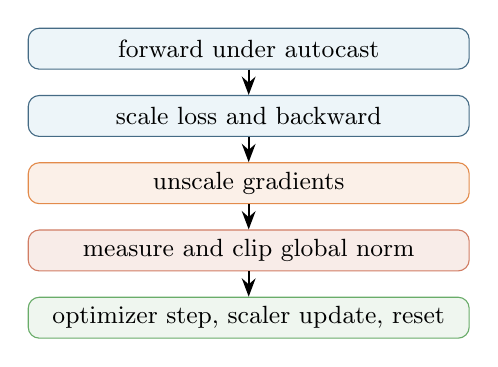
\begin{tikzpicture}[node distance=.32cm,every node/.style={font=\small},box/.style={draw=themebluedraw,fill=themebluebg,rounded corners,minimum width=5.6cm,minimum height=.52cm}]
    \node[box] (f) {forward under autocast};
    \node[box,below=of f] (b) {scale loss and backward};
    \node[box,fill=warningbg,draw=warningdraw,below=of b] (u) {unscale gradients};
    \node[box,fill=leafredbg,draw=leafreddraw,below=of u] (c) {measure and clip global norm};
    \node[box,fill=successbg,draw=successdraw,below=of c] (s) {optimizer step, scaler update, reset};
    \draw[-{Stealth},thick] (f)--(b);
    \draw[-{Stealth},thick] (b)--(u);
    \draw[-{Stealth},thick] (u)--(c);
    \draw[-{Stealth},thick] (c)--(s);
  \end{tikzpicture}
  \vfill
  \begin{alertblock}{Why unscale first?}
    Clipping scaled gradients measures a fictitious norm and changes the effective threshold.
  \end{alertblock}
\end{frame}

\begin{frame}{Global clipping preserves direction}
  \[
    \lVert g\rVert_2=\sqrt{\sum_i\lVert g_i\rVert_2^2}
  \]
  \[
    g_i \leftarrow g_i\cdot
    \min\!\left(1,\frac{M}{\lVert g\rVert_2+\epsilon}\right)
  \]
  \begin{itemize}
    \setlength{\itemsep}{8pt}
    \item All parameter gradients receive the same multiplier.
    \item Log the pre-clip norm and whether clipping activated.
    \item Frequent saturation is evidence of instability, not proof that clipping fixed it.
  \end{itemize}
\end{frame}

\begin{frame}{The scheduler counts optimizer updates}
  \begin{columns}[c]
    \begin{column}{0.55\linewidth}
      \scriptsize
      \[
        \eta_t=
        \begin{cases}
          \eta_{\max}\frac{t+1}{T_w+1} & t<T_w \\
          \eta_{\min}+\frac{1+\cos(\pi r)}{2}(\eta_{\max}-\eta_{\min}) & t\ge T_w
        \end{cases}
      \]
      where $r=(t-T_w)/(T_{\max}-T_w)$.
    \end{column}
    \begin{column}{0.41\linewidth}
      \begin{block}{Warmup}
        Limits early updates while activations and optimizer moments stabilize.
      \end{block}
      \begin{alertblock}{Silent failure}
        Stepping once per micro-batch compresses the schedule by factor $K$.
      \end{alertblock}
    \end{column}
  \end{columns}
\end{frame}

\begin{frame}{A catalog of loops that run but lie}
  \small
  \begin{tabular}{@{}>{\raggedright\arraybackslash}p{.30\linewidth}>{\raggedright\arraybackslash}p{.61\linewidth}@{}}
    \toprule
    Mistake & Consequence \\
    \midrule
    optimizer built before device move & optimizer may reference discarded parameters \\
    reset after backward & useful gradients are erased \\
    clipping before backward & clipping is a no-op \\
    clipping after step & the dangerous update already happened \\
    validation without no-grad & graphs consume memory needlessly \\
    log tensors instead of scalars & retained graphs create a memory leak \\
    omit \texttt{train()} after evaluation & dropout stays disabled \\
    \bottomrule
  \end{tabular}
\end{frame}

\checkpoint{repair the step}
  {Put these operations in order: clip, autocast forward, scaler update, scaled backward, unscale, optimizer step, scheduler step, gradient reset. Which operations occur only once per accumulated update?}

\section{Evaluation and recovery}

\begin{frame}{Evaluation changes mode, not parameters}
  \begin{columns}[c]
    \begin{column}{0.47\linewidth}
      \begin{block}{Required state}
        \texttt{model.eval()} changes dropout behavior.\\[4pt]
        \texttt{torch.no\_grad()} disables graph construction.
      \end{block}
    \end{column}
    \begin{column}{0.47\linewidth}
      \begin{block}{Stable estimate}
        Evaluate a fixed validation token budget. Aggregate loss by valid-token count.
      \end{block}
    \end{column}
  \end{columns}
  \begin{alertblock}{Return path}
    Call \texttt{model.train()} before the next training batch.
  \end{alertblock}
\end{frame}

\begin{frame}{An exact checkpoint captures the whole experiment state}
  \begin{columns}[t]
    \begin{column}{0.47\linewidth}
      \begin{block}{Numerical state}
        model parameters\\optimizer moments\\AMP scaler\\scheduler or global step
      \end{block}
    \end{column}
    \begin{column}{0.47\linewidth}
      \begin{block}{Data and randomness state}
        sampler position\\Python, NumPy, CPU and CUDA RNGs\\configuration and code version
      \end{block}
    \end{column}
  \end{columns}
  \vfill
  \begin{alertblock}{Recovery test}
    An uninterrupted run and a save-resume run should produce the same next batch, learning rate, loss, and update within the declared tolerance.
  \end{alertblock}
\end{frame}

\begin{frame}{A loop audit asks for evidence at boundaries}
  \begin{enumerate}
    \setlength{\itemsep}{8pt}
    \item Count valid tokens per update.
    \item Verify each parameter belongs to one optimizer group.
    \item Log learning rate and pre-clip gradient norm at update boundaries.
    \item Separate training loss, validation loss, throughput, and memory.
    \item Run the exact-resume comparison before long training.
  \end{enumerate}
\end{frame}

\takeaways
  {A training loop is a sequence of state transitions, not a four-line ritual.}
  {Accumulation changes the batch while clipping and scheduling remain update-level operations.}
  {AMP is safe only when gradients are unscaled before norm measurement and clipping.}
  {Validation and checkpoint recovery need explicit invariants of their own.}

\end{document}
